\documentclass[]{article}
\usepackage{lmodern}
\usepackage{amssymb,amsmath}
\usepackage{ifxetex,ifluatex}
\usepackage{fixltx2e} % provides \textsubscript
\ifnum 0\ifxetex 1\fi\ifluatex 1\fi=0 % if pdftex
  \usepackage[T1]{fontenc}
  \usepackage[utf8]{inputenc}
\else % if luatex or xelatex
  \ifxetex
    \usepackage{mathspec}
  \else
    \usepackage{fontspec}
  \fi
  \defaultfontfeatures{Ligatures=TeX,Scale=MatchLowercase}
\fi
% use upquote if available, for straight quotes in verbatim environments
\IfFileExists{upquote.sty}{\usepackage{upquote}}{}
% use microtype if available
\IfFileExists{microtype.sty}{%
\usepackage{microtype}
\UseMicrotypeSet[protrusion]{basicmath} % disable protrusion for tt fonts
}{}
\usepackage[margin=1in]{geometry}
\usepackage{hyperref}
\hypersetup{unicode=true,
            pdftitle={Computer Assisted Mass Appraisal - Residential},
            pdfborder={0 0 0},
            breaklinks=true}
\urlstyle{same}  % don't use monospace font for urls
\usepackage{color}
\usepackage{fancyvrb}
\newcommand{\VerbBar}{|}
\newcommand{\VERB}{\Verb[commandchars=\\\{\}]}
\DefineVerbatimEnvironment{Highlighting}{Verbatim}{commandchars=\\\{\}}
% Add ',fontsize=\small' for more characters per line
\usepackage{framed}
\definecolor{shadecolor}{RGB}{248,248,248}
\newenvironment{Shaded}{\begin{snugshade}}{\end{snugshade}}
\newcommand{\AlertTok}[1]{\textcolor[rgb]{0.94,0.16,0.16}{#1}}
\newcommand{\AnnotationTok}[1]{\textcolor[rgb]{0.56,0.35,0.01}{\textbf{\textit{#1}}}}
\newcommand{\AttributeTok}[1]{\textcolor[rgb]{0.77,0.63,0.00}{#1}}
\newcommand{\BaseNTok}[1]{\textcolor[rgb]{0.00,0.00,0.81}{#1}}
\newcommand{\BuiltInTok}[1]{#1}
\newcommand{\CharTok}[1]{\textcolor[rgb]{0.31,0.60,0.02}{#1}}
\newcommand{\CommentTok}[1]{\textcolor[rgb]{0.56,0.35,0.01}{\textit{#1}}}
\newcommand{\CommentVarTok}[1]{\textcolor[rgb]{0.56,0.35,0.01}{\textbf{\textit{#1}}}}
\newcommand{\ConstantTok}[1]{\textcolor[rgb]{0.00,0.00,0.00}{#1}}
\newcommand{\ControlFlowTok}[1]{\textcolor[rgb]{0.13,0.29,0.53}{\textbf{#1}}}
\newcommand{\DataTypeTok}[1]{\textcolor[rgb]{0.13,0.29,0.53}{#1}}
\newcommand{\DecValTok}[1]{\textcolor[rgb]{0.00,0.00,0.81}{#1}}
\newcommand{\DocumentationTok}[1]{\textcolor[rgb]{0.56,0.35,0.01}{\textbf{\textit{#1}}}}
\newcommand{\ErrorTok}[1]{\textcolor[rgb]{0.64,0.00,0.00}{\textbf{#1}}}
\newcommand{\ExtensionTok}[1]{#1}
\newcommand{\FloatTok}[1]{\textcolor[rgb]{0.00,0.00,0.81}{#1}}
\newcommand{\FunctionTok}[1]{\textcolor[rgb]{0.00,0.00,0.00}{#1}}
\newcommand{\ImportTok}[1]{#1}
\newcommand{\InformationTok}[1]{\textcolor[rgb]{0.56,0.35,0.01}{\textbf{\textit{#1}}}}
\newcommand{\KeywordTok}[1]{\textcolor[rgb]{0.13,0.29,0.53}{\textbf{#1}}}
\newcommand{\NormalTok}[1]{#1}
\newcommand{\OperatorTok}[1]{\textcolor[rgb]{0.81,0.36,0.00}{\textbf{#1}}}
\newcommand{\OtherTok}[1]{\textcolor[rgb]{0.56,0.35,0.01}{#1}}
\newcommand{\PreprocessorTok}[1]{\textcolor[rgb]{0.56,0.35,0.01}{\textit{#1}}}
\newcommand{\RegionMarkerTok}[1]{#1}
\newcommand{\SpecialCharTok}[1]{\textcolor[rgb]{0.00,0.00,0.00}{#1}}
\newcommand{\SpecialStringTok}[1]{\textcolor[rgb]{0.31,0.60,0.02}{#1}}
\newcommand{\StringTok}[1]{\textcolor[rgb]{0.31,0.60,0.02}{#1}}
\newcommand{\VariableTok}[1]{\textcolor[rgb]{0.00,0.00,0.00}{#1}}
\newcommand{\VerbatimStringTok}[1]{\textcolor[rgb]{0.31,0.60,0.02}{#1}}
\newcommand{\WarningTok}[1]{\textcolor[rgb]{0.56,0.35,0.01}{\textbf{\textit{#1}}}}
\usepackage{graphicx,grffile}
\makeatletter
\def\maxwidth{\ifdim\Gin@nat@width>\linewidth\linewidth\else\Gin@nat@width\fi}
\def\maxheight{\ifdim\Gin@nat@height>\textheight\textheight\else\Gin@nat@height\fi}
\makeatother
% Scale images if necessary, so that they will not overflow the page
% margins by default, and it is still possible to overwrite the defaults
% using explicit options in \includegraphics[width, height, ...]{}
\setkeys{Gin}{width=\maxwidth,height=\maxheight,keepaspectratio}
\IfFileExists{parskip.sty}{%
\usepackage{parskip}
}{% else
\setlength{\parindent}{0pt}
\setlength{\parskip}{6pt plus 2pt minus 1pt}
}
\setlength{\emergencystretch}{3em}  % prevent overfull lines
\providecommand{\tightlist}{%
  \setlength{\itemsep}{0pt}\setlength{\parskip}{0pt}}
\setcounter{secnumdepth}{0}
% Redefines (sub)paragraphs to behave more like sections
\ifx\paragraph\undefined\else
\let\oldparagraph\paragraph
\renewcommand{\paragraph}[1]{\oldparagraph{#1}\mbox{}}
\fi
\ifx\subparagraph\undefined\else
\let\oldsubparagraph\subparagraph
\renewcommand{\subparagraph}[1]{\oldsubparagraph{#1}\mbox{}}
\fi

%%% Use protect on footnotes to avoid problems with footnotes in titles
\let\rmarkdownfootnote\footnote%
\def\footnote{\protect\rmarkdownfootnote}

%%% Change title format to be more compact
\usepackage{titling}

% Create subtitle command for use in maketitle
\newcommand{\subtitle}[1]{
  \posttitle{
    \begin{center}\large#1\end{center}
    }
}

\setlength{\droptitle}{-2em}
  \title{Computer Assisted Mass Appraisal - Residential}
  \pretitle{\vspace{\droptitle}\centering\huge}
  \posttitle{\par}
  \author{}
  \preauthor{}\postauthor{}
  \date{}
  \predate{}\postdate{}


\begin{document}
\maketitle

{
\setcounter{tocdepth}{2}
\tableofcontents
}
\hypertarget{introduction.}{%
\subsection{Introduction.}\label{introduction.}}

\emph{Is it possible to create a predictive model to predict sale price
of residential properties in DC area?}

District of Columbia shares hundreds of datasets which can be used for
analysis and planning by different agencies and public.

Computer Assisted Mass Appraisal (CAMA) database is one the interesting
datasets with residential appraisals. The dataset contains attribution
on housing characteristics for residential properties, and was created
as part of the DC Geographic Information System (DC GIS) for the DC
Office of the Chief Technology Officer (OCTO) and participating D.C.
government agencies.\\
For more details see
\url{http://opendata.dc.gov/datasets/computer-assisted-mass-appraisal-residential}.

Technical aspects expected to be showcased in this project are. 1.
Exloratory Data Analysis. 2. Data wrangling. 3. Data merging. 4. Visual
analysis of data. 5. Regression models. 6. Presentation tools.

\hypertarget{data-wrangling.}{%
\subsection{Data wrangling.}\label{data-wrangling.}}

\hypertarget{load-libraries}{%
\subsubsection{Load Libraries}\label{load-libraries}}

\begin{Shaded}
\begin{Highlighting}[]
\KeywordTok{library}\NormalTok{(readr)}
\KeywordTok{library}\NormalTok{(ggplot2)}
\KeywordTok{library}\NormalTok{(tibble)}
\KeywordTok{library}\NormalTok{(dplyr)}
\end{Highlighting}
\end{Shaded}

\begin{verbatim}
## 
## Attaching package: 'dplyr'
\end{verbatim}

\begin{verbatim}
## The following objects are masked from 'package:stats':
## 
##     filter, lag
\end{verbatim}

\begin{verbatim}
## The following objects are masked from 'package:base':
## 
##     intersect, setdiff, setequal, union
\end{verbatim}

\begin{Shaded}
\begin{Highlighting}[]
\KeywordTok{library}\NormalTok{(tidyr)}
\KeywordTok{library}\NormalTok{(lubridate)}
\end{Highlighting}
\end{Shaded}

\begin{verbatim}
## 
## Attaching package: 'lubridate'
\end{verbatim}

\begin{verbatim}
## The following object is masked from 'package:base':
## 
##     date
\end{verbatim}

\begin{Shaded}
\begin{Highlighting}[]
\KeywordTok{library}\NormalTok{(GGally)}
\end{Highlighting}
\end{Shaded}

\begin{verbatim}
## 
## Attaching package: 'GGally'
\end{verbatim}

\begin{verbatim}
## The following object is masked from 'package:dplyr':
## 
##     nasa
\end{verbatim}

\hypertarget{data-load.}{%
\subsubsection{Data Load.}\label{data-load.}}

\begin{Shaded}
\begin{Highlighting}[]
\NormalTok{residential_raw_df <-}\StringTok{ }\KeywordTok{read_csv}\NormalTok{(}\StringTok{'Data/Computer_Assisted_Mass_Appraisal__Residential.csv'}\NormalTok{)}
\end{Highlighting}
\end{Shaded}

\begin{verbatim}
## Parsed with column specification:
## cols(
##   .default = col_integer(),
##   SSL = col_character(),
##   HEAT_D = col_character(),
##   AC = col_character(),
##   STORIES = col_double(),
##   SALEDATE = col_datetime(format = ""),
##   QUALIFIED = col_character(),
##   STYLE_D = col_character(),
##   STRUCT_D = col_character(),
##   GRADE_D = col_character(),
##   CNDTN_D = col_character(),
##   EXTWALL_D = col_character(),
##   ROOF_D = col_character(),
##   INTWALL_D = col_character(),
##   GIS_LAST_MOD_DTTM = col_datetime(format = "")
## )
\end{verbatim}

\begin{verbatim}
## See spec(...) for full column specifications.
\end{verbatim}

\begin{Shaded}
\begin{Highlighting}[]
\KeywordTok{glimpse}\NormalTok{(residential_raw_df)}
\end{Highlighting}
\end{Shaded}

\begin{verbatim}
## Observations: 107,237
## Variables: 39
## $ OBJECTID          <int> 1001, 1002, 1003, 1004, 1005, 1006, 1007, 10...
## $ SSL               <chr> "0193    0088", "0193    0090", "0193    009...
## $ BATHRM            <int> 1, 4, 3, 4, 2, 2, 3, 2, 1, 2, 1, 1, 2, 2, 2,...
## $ HF_BATHRM         <int> 0, 0, 0, 1, 1, 0, 0, 1, 1, 0, 0, 1, 0, 1, 0,...
## $ HEAT              <int> 1, 13, 7, 8, 13, 13, 7, 7, 7, 1, 13, 13, 7, ...
## $ HEAT_D            <chr> "Forced Air", "Hot Water Rad", "Warm Cool", ...
## $ AC                <chr> "N", "Y", "Y", "Y", "N", "N", "Y", "Y", "Y",...
## $ NUM_UNITS         <int> 1, 4, 2, 2, 2, 2, 2, 2, 1, 2, 1, 1, 2, 2, 2,...
## $ ROOMS             <int> 9, 16, 8, 6, 10, 7, 6, 7, 7, 9, 7, 11, 8, 10...
## $ BEDRM             <int> 3, 4, 3, 4, 5, 3, 3, 3, 3, 4, 4, 3, 4, 5, 5,...
## $ AYB               <int> 1860, 1870, 1870, 1870, 1870, 1870, 1895, 18...
## $ YR_RMDL           <int> NA, 2005, NA, 2014, NA, NA, NA, 1974, NA, NA...
## $ EYB               <int> 1960, 1978, 1960, 1982, 1960, 1957, 1986, 19...
## $ STORIES           <dbl> 2, 4, 3, 2, 2, 2, 2, 2, 2, 2, 2, 2, 2, 2, 2,...
## $ SALEDATE          <dttm> 2006-08-23, 2015-12-16, 2003-09-04, 2009-07...
## $ PRICE             <int> 0, 1525000, 0, 1515000, NA, NA, 1380000, NA,...
## $ QUALIFIED         <chr> "U", "Q", "U", "U", "U", "U", "Q", "U", "U",...
## $ SALE_NUM          <int> 1, 4, 1, 1, 1, 1, 6, 1, 4, 1, 1, 1, 1, 1, 1,...
## $ GBA               <int> 1168, 2784, 2035, 1610, 1422, 1190, 1218, 12...
## $ BLDG_NUM          <int> 1, 1, 1, 1, 1, 1, 1, 1, 1, 1, 1, 1, 1, 1, 1,...
## $ STYLE             <int> 4, 10, 7, 4, 4, 4, 4, 4, 4, 4, 4, 4, 4, 4, 4...
## $ STYLE_D           <chr> "2 Story", "4 Story", "3 Story", "2 Story", ...
## $ STRUCT            <int> 7, 7, 7, 7, 7, 7, 7, 7, 6, 7, 7, 7, 6, 7, 7,...
## $ STRUCT_D          <chr> "Row Inside", "Row Inside", "Row Inside", "R...
## $ GRADE             <int> 5, 7, 5, 5, 5, 4, 5, 5, 4, 5, 5, 5, 5, 5, 5,...
## $ GRADE_D           <chr> "Good Quality", "Excellent", "Good Quality",...
## $ CNDTN             <int> 2, 4, 4, 4, 4, 4, 5, 4, 3, 3, 3, 3, 3, 3, 4,...
## $ CNDTN_D           <chr> "Fair", "Good", "Good", "Good", "Good", "Goo...
## $ EXTWALL           <int> 14, 21, 14, 14, 14, 14, 14, 14, 14, 14, 14, ...
## $ EXTWALL_D         <chr> "Common Brick", "Brick/Stucco", "Common Bric...
## $ ROOF              <int> 2, 2, 6, 2, 6, 6, 2, 6, 6, 6, 6, 6, 6, 2, 6,...
## $ ROOF_D            <chr> "Built Up", "Built Up", "Metal- Sms", "Built...
## $ INTWALL           <int> 6, 6, 6, 6, 6, 6, 6, 3, 6, 6, 6, 6, 6, 6, 6,...
## $ INTWALL_D         <chr> "Hardwood", "Hardwood", "Hardwood", "Hardwoo...
## $ KITCHENS          <int> 1, 4, 2, 2, 2, 2, 2, 2, 1, 2, 1, 1, 2, 2, 2,...
## $ FIREPLACES        <int> 0, 0, 2, 2, 0, 2, 2, 0, 0, 1, 0, 1, 0, 1, 2,...
## $ USECODE           <int> 11, 24, 24, 24, 24, 24, 24, 24, 11, 24, 11, ...
## $ LANDAREA          <int> 707, 771, 1647, 1647, 1647, 1647, 1647, 1647...
## $ GIS_LAST_MOD_DTTM <dttm> 2018-08-12 20:22:19, 2018-08-12 20:22:19, 2...
\end{verbatim}

Dataset has 39 variables and 107,237 observations. Create a new df
called cleaned version.\\
Object ID is serial number and last variable the db updated date. These
are of no importance for data analysis. Let's exclude these from the
data frame.

\begin{Shaded}
\begin{Highlighting}[]
\NormalTok{residential_clean_df <-}\StringTok{ }\NormalTok{residential_raw_df }\OperatorTok
\StringTok{  }\KeywordTok{subset}\NormalTok{( }\DataTypeTok{select =} \OperatorTok{-}\KeywordTok{c}\NormalTok{(OBJECTID, GIS_LAST_MOD_DTTM))}
\end{Highlighting}
\end{Shaded}

\hypertarget{bathrooms.}{%
\subsubsection{Bathrooms.}\label{bathrooms.}}

HF\_BATHRM can be merged with BATHRM to create BATHROOMS\_TOT variable.

\begin{Shaded}
\begin{Highlighting}[]
\NormalTok{residential_clean_df <-}\StringTok{ }\NormalTok{residential_clean_df }\OperatorTok
\StringTok{  }\KeywordTok{mutate}\NormalTok{(}\DataTypeTok{BATHROOM_TOTAL =}\NormalTok{ BATHRM }\OperatorTok{+}\StringTok{ }\FloatTok{0.5}\OperatorTok{*}\NormalTok{HF_BATHRM) }
\KeywordTok{summary}\NormalTok{(residential_clean_df}\OperatorTok{$}\NormalTok{BATHROOM_TOTAL)}
\end{Highlighting}
\end{Shaded}

\begin{verbatim}
##    Min. 1st Qu.  Median    Mean 3rd Qu.    Max.    NA's 
##   0.000   1.500   2.000   2.338   3.000  24.000     113
\end{verbatim}

Check out the 113 records which have NA for BATHROOM\_TOT

\begin{Shaded}
\begin{Highlighting}[]
\NormalTok{residential_clean_df }\OperatorTok
\StringTok{  }\KeywordTok{filter}\NormalTok{(}\KeywordTok{is.na}\NormalTok{(BATHROOM_TOTAL))}
\end{Highlighting}
\end{Shaded}

\begin{verbatim}
## # A tibble: 113 x 38
##    SSL     BATHRM HF_BATHRM  HEAT HEAT_D AC    NUM_UNITS ROOMS BEDRM   AYB
##    <chr>    <int>     <int> <int> <chr>  <chr>     <int> <int> <int> <int>
##  1 0070  ~     NA        NA    NA <NA>   <NA>         NA    NA    NA  2019
##  2 0429  ~     NA        NA    NA <NA>   <NA>         NA    NA    NA  2019
##  3 0429  ~     NA        NA    NA <NA>   <NA>         NA    NA    NA  2019
##  4 0869  ~      5        NA     1 Force~ Y             5    12     5  1900
##  5 1047  ~     NA        NA    NA <NA>   <NA>         NA    NA    NA  2019
##  6 1047  ~     NA        NA    NA <NA>   <NA>         NA    NA    NA  2019
##  7 1047  ~     NA        NA    NA <NA>   <NA>         NA    NA    NA  2019
##  8 1047  ~     NA        NA    NA <NA>   <NA>         NA    NA    NA  2019
##  9 1047  ~     NA        NA    NA <NA>   <NA>         NA    NA    NA  2019
## 10 1047  ~     NA        NA    NA <NA>   <NA>         NA    NA    NA  2019
## # ... with 103 more rows, and 28 more variables: YR_RMDL <int>, EYB <int>,
## #   STORIES <dbl>, SALEDATE <dttm>, PRICE <int>, QUALIFIED <chr>,
## #   SALE_NUM <int>, GBA <int>, BLDG_NUM <int>, STYLE <int>, STYLE_D <chr>,
## #   STRUCT <int>, STRUCT_D <chr>, GRADE <int>, GRADE_D <chr>, CNDTN <int>,
## #   CNDTN_D <chr>, EXTWALL <int>, EXTWALL_D <chr>, ROOF <int>,
## #   ROOF_D <chr>, INTWALL <int>, INTWALL_D <chr>, KITCHENS <int>,
## #   FIREPLACES <int>, USECODE <int>, LANDAREA <int>, BATHROOM_TOTAL <dbl>
\end{verbatim}

Only record with SSL `0869 0027' has bathroom 5 and hf\_bathroom as na.
Total bath room can be imputed to 5. Rest of the records have na in
majority of the columns. These records need to be deleted.

\begin{Shaded}
\begin{Highlighting}[]
\NormalTok{residential_clean_df[residential_clean_df[}\StringTok{'SSL'}\NormalTok{] }\OperatorTok{==}\StringTok{ '0869    0027'}\NormalTok{,}\StringTok{'BATHROOM_TOTAL'}\NormalTok{] =}\StringTok{ }\DecValTok{5}
\NormalTok{residential_clean_df <-}\StringTok{ }\NormalTok{residential_clean_df }\OperatorTok
\StringTok{  }\KeywordTok{filter}\NormalTok{(}\OperatorTok{!}\KeywordTok{is.na}\NormalTok{(BATHROOM_TOTAL)) }\OperatorTok
\StringTok{  }\KeywordTok{select}\NormalTok{(}\OperatorTok{-}\NormalTok{BATHRM, }\OperatorTok{-}\NormalTok{HF_BATHRM)}
\end{Highlighting}
\end{Shaded}

\hypertarget{heating.}{%
\subsubsection{Heating.}\label{heating.}}

Analyse heating related columns.

\begin{Shaded}
\begin{Highlighting}[]
\KeywordTok{table}\NormalTok{(residential_clean_df}\OperatorTok{$}\NormalTok{HEAT_D, residential_clean_df}\OperatorTok{$}\NormalTok{HEAT)}
\end{Highlighting}
\end{Shaded}

\begin{verbatim}
##                 
##                      0     1     2     3     4     5     6     7     8
##   Air Exchng         0     0     0     0     0     0     0     0     0
##   Air-Oil            0     0    98     0     0     0     0     0     0
##   Elec Base Brd      0     0     0     0     0   108     0     0     0
##   Electric Rad       0     0     0     0    76     0     0     0     0
##   Evp Cool           0     0     0     0     0     0     0     0     0
##   Forced Air         0 32407     0     0     0     0     0     0     0
##   Gravity Furnac     0     0     0     0     0     0     0     0     0
##   Hot Water Rad      0     0     0     0     0     0     0     0     0
##   Ht Pump            0     0     0     0     0     0     0     0   946
##   Ind Unit           0     0     0     0     0     0     0     0     0
##   No Data           61     0     0     0     0     0     0     0     0
##   Wall Furnace       0     0     0   234     0     0     0     0     0
##   Warm Cool          0     0     0     0     0     0     0 28756     0
##   Water Base Brd     0     0     0     0     0     0   187     0     0
##                 
##                      9    10    11    12    13
##   Air Exchng         0    36     0     0     0
##   Air-Oil            0     0     0     0     0
##   Elec Base Brd      0     0     0     0     0
##   Electric Rad       0     0     0     0     0
##   Evp Cool          36     0     0     0     0
##   Forced Air         0     0     0     0     0
##   Gravity Furnac     0     0   139     0     0
##   Hot Water Rad      0     0     0     0 44024
##   Ht Pump            0     0     0     0     0
##   Ind Unit           0     0     0    17     0
##   No Data            0     0     0     0     0
##   Wall Furnace       0     0     0     0     0
##   Warm Cool          0     0     0     0     0
##   Water Base Brd     0     0     0     0     0
\end{verbatim}

There are 13 categories of heating and each of them are coded in HEAT
column. There are 61 records with `No Data'. There is no discernible
pattern here. Need to get back later. HEAT column needs to be factor and
heat\_d can be deleted.

\begin{Shaded}
\begin{Highlighting}[]
\NormalTok{residential_clean_df <-}\StringTok{ }\NormalTok{residential_clean_df }\OperatorTok\StringTok{ }
\StringTok{  }\KeywordTok{mutate}\NormalTok{(}\DataTypeTok{HEAT =} \KeywordTok{as.factor}\NormalTok{(HEAT)) }\OperatorTok
\StringTok{  }\KeywordTok{select}\NormalTok{(}\OperatorTok{-}\NormalTok{HEAT_D)}
\end{Highlighting}
\end{Shaded}

\hypertarget{air-condition.}{%
\subsubsection{Air condition.}\label{air-condition.}}

AC column has N, Y and 0 values. o is absence of AC which can be coded
back to `N'.

\begin{Shaded}
\begin{Highlighting}[]
\NormalTok{ residential_clean_df <-}\StringTok{ }\NormalTok{residential_clean_df }\OperatorTok
\StringTok{  }\KeywordTok{mutate}\NormalTok{(}\DataTypeTok{AC =} \KeywordTok{if_else}\NormalTok{(AC }\OperatorTok{==}\StringTok{ '0'}\NormalTok{, }\StringTok{'N'}\NormalTok{,AC))}
\CommentTok{# code N to 0 and Y to 1.}
\NormalTok{ residential_clean_df <-}\StringTok{ }\NormalTok{residential_clean_df }\OperatorTok
\StringTok{  }\KeywordTok{mutate}\NormalTok{(}\DataTypeTok{AC =} \KeywordTok{if_else}\NormalTok{(AC }\OperatorTok{==}\StringTok{ 'N'}\NormalTok{, }\DecValTok{0}\NormalTok{,}\DecValTok{1}\NormalTok{))}
\end{Highlighting}
\end{Shaded}

\hypertarget{building-number.}{%
\subsubsection{Building Number.}\label{building-number.}}

Building number. As per the meta data For parcels where multiple
buildings exist, the primary building (such as the main residence) is
assigned BLDG\_NUM = 1. The other buildings or structures have BLDG\_NUM
values in random sequential order. So BLDG\_NUM is just a number of
building on a parcel which does not have any significance for the
analysis. Removing the column.

\begin{Shaded}
\begin{Highlighting}[]
\NormalTok{residential_clean_df <-}\StringTok{ }\NormalTok{residential_clean_df }\OperatorTok
\StringTok{  }\KeywordTok{select}\NormalTok{(}\OperatorTok{-}\NormalTok{BLDG_NUM)}
\end{Highlighting}
\end{Shaded}

\hypertarget{feature-descriptions.}{%
\subsubsection{Feature Descriptions.}\label{feature-descriptions.}}

All below attributes have descriptions and codes. Tabulate the data for
any obvious errors and remove the description columns.

\begin{Shaded}
\begin{Highlighting}[]
\KeywordTok{table}\NormalTok{(residential_clean_df}\OperatorTok{$}\NormalTok{STYLE_D, residential_clean_df}\OperatorTok{$}\NormalTok{STYLE)}
\end{Highlighting}
\end{Shaded}

\begin{verbatim}
##                  
##                       0     1     2     3     4     5     6     7     8
##   1 Story             0  4439     0     0     0     0     0     0     0
##   1.5 Story Fin       0     0     0  2665     0     0     0     0     0
##   1.5 Story Unfin     0     0   112     0     0     0     0     0     0
##   2 Story             0     0     0     0 81451     0     0     0     0
##   2.5 Story Fin       0     0     0     0     0     0  7015     0     0
##   2.5 Story Unfin     0     0     0     0     0   732     0     0     0
##   3 Story             0     0     0     0     0     0     0  9508     0
##   3.5 Story Fin       0     0     0     0     0     0     0     0     0
##   3.5 Story Unfin     0     0     0     0     0     0     0     0     8
##   4 Story             0     0     0     0     0     0     0     0     0
##   4.5 Story Fin       0     0     0     0     0     0     0     0     0
##   4.5 Story Unfin     0     0     0     0     0     0     0     0     0
##   Bi-Level            0     0     0     0     0     0     0     0     0
##   Default            68     0     0     0     0     0     0     0     0
##   Outbuildings        0     0     0     0     0     0     0     0     0
##   Split Foyer         0     0     0     0     0     0     0     0     0
##   Split Level         0     0     0     0     0     0     0     0     0
##   Vacant              0     0     0     0     0     0     0     0     0
##                  
##                       9    10    11    12    13    14    15    94    99
##   1 Story             0     0     0     0     0     0     0     0     0
##   1.5 Story Fin       0     0     0     0     0     0     0     0     0
##   1.5 Story Unfin     0     0     0     0     0     0     0     0     0
##   2 Story             0     0     0     0     0     0     0     0     0
##   2.5 Story Fin       0     0     0     0     0     0     0     0     0
##   2.5 Story Unfin     0     0     0     0     0     0     0     0     0
##   3 Story             0     0     0     0     0     0     0     0     0
##   3.5 Story Fin     134     0     0     0     0     0     0     0     0
##   3.5 Story Unfin     0     0     0     0     0     0     0     0     0
##   4 Story             0   371     0     0     0     0     0     0     0
##   4.5 Story Fin       0     0     0    13     0     0     0     0     0
##   4.5 Story Unfin     0     0     2     0     0     0     0     0     0
##   Bi-Level            0     0     0     0    19     0     0     0     0
##   Default             0     0     0     0     0     0     0     0     0
##   Outbuildings        0     0     0     0     0     0     0     1     0
##   Split Foyer         0     0     0     0     0     0   281     0     0
##   Split Level         0     0     0     0     0   304     0     0     0
##   Vacant              0     0     0     0     0     0     0     0     2
\end{verbatim}

\begin{Shaded}
\begin{Highlighting}[]
\KeywordTok{table}\NormalTok{(residential_clean_df}\OperatorTok{$}\NormalTok{STRUCT_D, residential_clean_df}\OperatorTok{$}\NormalTok{STRUCT)}
\end{Highlighting}
\end{Shaded}

\begin{verbatim}
##                
##                     0     1     2     4     5     6     7     8    12
##   Condo             0     0     0     0     0     0     0     0     1
##   Default          26     0     0     0     0     0     0     0     0
##   Multi             0     0  4745     0     0     0     0     0     0
##   Row End           0     0     0     0     0 12278     0     0     0
##   Row Inside        0     0     0     0     0     0 40782     0     0
##   Semi-Detached     0     0     0     0     0     0     0 16828     0
##   Single            0 32158     0     0     0     0     0     0     0
##   Town End          0     0     0    85     0     0     0     0     0
##   Town Inside       0     0     0     0   218     0     0     0     0
##   Vacant Land       0     0     0     0     0     0     0     0     0
##                
##                    13
##   Condo             0
##   Default           0
##   Multi             0
##   Row End           0
##   Row Inside        0
##   Semi-Detached     0
##   Single            0
##   Town End          0
##   Town Inside       0
##   Vacant Land       4
\end{verbatim}

\begin{Shaded}
\begin{Highlighting}[]
\KeywordTok{table}\NormalTok{(residential_clean_df}\OperatorTok{$}\NormalTok{GRADE_D, residential_clean_df}\OperatorTok{$}\NormalTok{GRADE)}
\end{Highlighting}
\end{Shaded}

\begin{verbatim}
##                
##                     0     1     2     3     4     5     6     7     8
##   Above Average     0     0     0     0 32214     0     0     0     0
##   Average           0     0     0 37576     0     0     0     0     0
##   Excellent         0     0     0     0     0     0     0  3400     0
##   Exceptional-A     0     0     0     0     0     0     0     0     0
##   Exceptional-B     0     0     0     0     0     0     0     0     0
##   Exceptional-C     0     0     0     0     0     0     0     0     0
##   Exceptional-D     0     0     0     0     0     0     0     0     0
##   Fair Quality      0     0   151     0     0     0     0     0     0
##   Good Quality      0     0     0     0     0 20857     0     0     0
##   Low Quality       0     6     0     0     0     0     0     0     0
##   No Data          20     0     0     0     0     0     0     0     0
##   Superior          0     0     0     0     0     0     0     0  2635
##   Very Good         0     0     0     0     0     0  8999     0     0
##                
##                     9    10    11    12
##   Above Average     0     0     0     0
##   Average           0     0     0     0
##   Excellent         0     0     0     0
##   Exceptional-A   820     0     0     0
##   Exceptional-B     0   278     0     0
##   Exceptional-C     0     0    92     0
##   Exceptional-D     0     0     0    77
##   Fair Quality      0     0     0     0
##   Good Quality      0     0     0     0
##   Low Quality       0     0     0     0
##   No Data           0     0     0     0
##   Superior          0     0     0     0
##   Very Good         0     0     0     0
\end{verbatim}

\begin{Shaded}
\begin{Highlighting}[]
\KeywordTok{table}\NormalTok{(residential_clean_df}\OperatorTok{$}\NormalTok{CNDTN_D, residential_clean_df}\OperatorTok{$}\NormalTok{CNDTN)}
\end{Highlighting}
\end{Shaded}

\begin{verbatim}
##            
##                 0     1     2     3     4     5     6
##   Average       0     0     0 58408     0     0     0
##   Default      20     0     0     0     0     0     0
##   Excellent     0     0     0     0     0     0  1350
##   Fair          0     0  1329     0     0     0     0
##   Good          0     0     0     0 37679     0     0
##   Poor          0   176     0     0     0     0     0
##   Very Good     0     0     0     0     0  8163     0
\end{verbatim}

\begin{Shaded}
\begin{Highlighting}[]
\KeywordTok{table}\NormalTok{(residential_clean_df}\OperatorTok{$}\NormalTok{EXTWALL_D, residential_clean_df}\OperatorTok{$}\NormalTok{EXTWALL)}
\end{Highlighting}
\end{Shaded}

\begin{verbatim}
##                 
##                      0     1     2     3     4     5     6     7     8
##   Adobe              0     0     0     0     0     0     0     0     0
##   Aluminum           0     0     0     0     0     0     0     0     0
##   Brick Veneer       0     0     0     0     0     0     0     0     0
##   Brick/Siding       0     0     0     0     0     0     0     0     0
##   Brick/Stone        0     0     0     0     0     0     0     0     0
##   Brick/Stucco       0     0     0     0     0     0     0     0     0
##   Common Brick       0     0     0     0     0     0     0     0     0
##   Concrete           0     0     0     0     0     0     0     0     0
##   Concrete Block     0     0     0     0     0     0     0     0     0
##   Default           32     0     0     0     0     0     0     0     0
##   Face Brick         0     0     0     0     0     0     0     0     0
##   Hardboard          0     0   123     0     0     0     0     0     0
##   Metal Siding       0     0     0    69     0     0     0     0     0
##   Plywood            0    15     0     0     0     0     0     0     0
##   Rustic Log         0     0     0     0     0     0     0     0     0
##   Shingle            0     0     0     0     0     0     0  1184     0
##   SPlaster           0     0     0     0     0     0     0     0     1
##   Stone              0     0     0     0     0     0     0     0     0
##   Stone Veneer       0     0     0     0     0     0     0     0     0
##   Stone/Siding       0     0     0     0     0     0     0     0     0
##   Stone/Stucco       0     0     0     0     0     0     0     0     0
##   Stucco             0     0     0     0     0  3223     0     0     0
##   Stucco Block       0     0     0     0     0     0     0     0     0
##   Vinyl Siding       0     0     0     0  5317     0     0     0     0
##   Wood Siding        0     0     0     0     0     0  4567     0     0
##                 
##                      9    10    11    12    13    14    15    16    17
##   Adobe              0     0     0     0     0     0     0     2     0
##   Aluminum           0     0     0     0     0     0     0     0     0
##   Brick Veneer       0  1071     0     0     0     0     0     0     0
##   Brick/Siding       0     0     0     0     0     0     0     0     0
##   Brick/Stone        0     0     0     0     0     0     0     0     0
##   Brick/Stucco       0     0     0     0     0     0     0     0     0
##   Common Brick       0     0     0     0     0 81376     0     0     0
##   Concrete           0     0     0     0     0     0     0     0     0
##   Concrete Block     0     0     0    54     0     0     0     0     0
##   Default            0     0     0     0     0     0     0     0     0
##   Face Brick         0     0     0     0     0     0   523     0     0
##   Hardboard          0     0     0     0     0     0     0     0     0
##   Metal Siding       0     0     0     0     0     0     0     0     0
##   Plywood            0     0     0     0     0     0     0     0     0
##   Rustic Log         1     0     0     0     0     0     0     0     0
##   Shingle            0     0     0     0     0     0     0     0     0
##   SPlaster           0     0     0     0     0     0     0     0     0
##   Stone              0     0     0     0     0     0     0     0   748
##   Stone Veneer       0     0   257     0     0     0     0     0     0
##   Stone/Siding       0     0     0     0     0     0     0     0     0
##   Stone/Stucco       0     0     0     0     0     0     0     0     0
##   Stucco             0     0     0     0     0     0     0     0     0
##   Stucco Block       0     0     0     0    53     0     0     0     0
##   Vinyl Siding       0     0     0     0     0     0     0     0     0
##   Wood Siding        0     0     0     0     0     0     0     0     0
##                 
##                     18    19    20    21    22    23    24
##   Adobe              0     0     0     0     0     0     0
##   Aluminum           0   954     0     0     0     0     0
##   Brick Veneer       0     0     0     0     0     0     0
##   Brick/Siding       0     0     0     0  5590     0     0
##   Brick/Stone        0     0   628     0     0     0     0
##   Brick/Stucco       0     0     0   674     0     0     0
##   Common Brick       0     0     0     0     0     0     0
##   Concrete          83     0     0     0     0     0     0
##   Concrete Block     0     0     0     0     0     0     0
##   Default            0     0     0     0     0     0     0
##   Face Brick         0     0     0     0     0     0     0
##   Hardboard          0     0     0     0     0     0     0
##   Metal Siding       0     0     0     0     0     0     0
##   Plywood            0     0     0     0     0     0     0
##   Rustic Log         0     0     0     0     0     0     0
##   Shingle            0     0     0     0     0     0     0
##   SPlaster           0     0     0     0     0     0     0
##   Stone              0     0     0     0     0     0     0
##   Stone Veneer       0     0     0     0     0     0     0
##   Stone/Siding       0     0     0     0     0     0   341
##   Stone/Stucco       0     0     0     0     0   239     0
##   Stucco             0     0     0     0     0     0     0
##   Stucco Block       0     0     0     0     0     0     0
##   Vinyl Siding       0     0     0     0     0     0     0
##   Wood Siding        0     0     0     0     0     0     0
\end{verbatim}

\begin{Shaded}
\begin{Highlighting}[]
\KeywordTok{table}\NormalTok{(residential_clean_df}\OperatorTok{$}\NormalTok{ROOF_D, residential_clean_df}\OperatorTok{$}\NormalTok{ROOF)}
\end{Highlighting}
\end{Shaded}

\begin{verbatim}
##                 
##                      0     1     2     3     4     5     6     7     8
##   Built Up           0     0 31557     0     0     0     0     0     0
##   Clay Tile          0     0     0     0     0     0     0     0     0
##   Comp Shingle       0 30409     0     0     0     0     0     0     0
##   Composition Ro     0     0     0     0     0     0     0     0   106
##   Concrete           0     0     0     0     0     0     0     0     0
##   Concrete Tile      0     0     0     0     0     0     0     0     0
##   Metal- Cpr         0     0     0     0     0     0     0    41     0
##   Metal- Pre         0     0     0     0     0   253     0     0     0
##   Metal- Sms         0     0     0     0     0     0 30064     0     0
##   Neopren            0     0     0     0     0     0     0     0     0
##   Shake              0     0     0     0   912     0     0     0     0
##   Shingle            0     0     0   435     0     0     0     0     0
##   Slate              0     0     0     0     0     0     0     0     0
##   Typical          237     0     0     0     0     0     0     0     0
##   Water Proof        0     0     0     0     0     0     0     0     0
##   Wood- FS           0     0     0     0     0     0     0     0     0
##                 
##                      9    10    11    12    13    14    15
##   Built Up           0     0     0     0     0     0     0
##   Clay Tile          0   657     0     0     0     0     0
##   Comp Shingle       0     0     0     0     0     0     0
##   Composition Ro     0     0     0     0     0     0     0
##   Concrete           0     0     0     4     0     0     0
##   Concrete Tile     17     0     0     0     0     0     0
##   Metal- Cpr         0     0     0     0     0     0     0
##   Metal- Pre         0     0     0     0     0     0     0
##   Metal- Sms         0     0     0     0     0     0     0
##   Neopren            0     0     0     0  1258     0     0
##   Shake              0     0     0     0     0     0     0
##   Shingle            0     0     0     0     0     0     0
##   Slate              0     0 11159     0     0     0     0
##   Typical            0     0     0     0     0     0     0
##   Water Proof        0     0     0     0     0     9     0
##   Wood- FS           0     0     0     0     0     0     7
\end{verbatim}

\begin{Shaded}
\begin{Highlighting}[]
\KeywordTok{table}\NormalTok{(residential_clean_df}\OperatorTok{$}\NormalTok{INTWALL_D, residential_clean_df}\OperatorTok{$}\NormalTok{INTWALL)}
\end{Highlighting}
\end{Shaded}

\begin{verbatim}
##                
##                     0     1     2     3     4     5     6     7     8
##   Carpet            0     0  3591     0     0     0     0     0     0
##   Ceramic Tile      0     0     0     0    50     0     0     0     0
##   Default         121     0     0     0     0     0     0     0     0
##   Hardwood          0     0     0     0     0     0 83967     0     0
##   Hardwood/Carp     0     0     0     0     0     0     0     0     0
##   Lt Concrete       0     0     0     0     0     0     0     0     0
##   Parquet           0     0     0     0     0     0     0    19     0
##   Resiliant         0    15     0     0     0     0     0     0     0
##   Terrazo           0     0     0     0     0     6     0     0     0
##   Vinyl Comp        0     0     0     0     0     0     0     0    30
##   Vinyl Sheet       0     0     0     0     0     0     0     0     0
##   Wood Floor        0     0     0  8220     0     0     0     0     0
##                
##                     9    10    11
##   Carpet            0     0     0
##   Ceramic Tile      0     0     0
##   Default           0     0     0
##   Hardwood          0     0     0
##   Hardwood/Carp     0     0 10952
##   Lt Concrete       0   141     0
##   Parquet           0     0     0
##   Resiliant         0     0     0
##   Terrazo           0     0     0
##   Vinyl Comp        0     0     0
##   Vinyl Sheet      13     0     0
##   Wood Floor        0     0     0
\end{verbatim}

\begin{Shaded}
\begin{Highlighting}[]
\CommentTok{# There are no obvious data errors. Removing the descriptions and coding the rest columns as factors.}
\NormalTok{residential_clean_df <-}\StringTok{ }\NormalTok{residential_clean_df }\OperatorTok
\StringTok{  }\KeywordTok{select}\NormalTok{(}\OperatorTok{-}\NormalTok{STYLE_D, }\OperatorTok{-}\NormalTok{STRUCT_D,}\OperatorTok{-}\NormalTok{GRADE_D,}\OperatorTok{-}\NormalTok{CNDTN_D,}\OperatorTok{-}\NormalTok{EXTWALL_D,}\OperatorTok{-}\NormalTok{ROOF_D,}\OperatorTok{-}\NormalTok{INTWALL_D) }\OperatorTok
\StringTok{  }\KeywordTok{mutate}\NormalTok{(}\DataTypeTok{STYLE =} \KeywordTok{as.factor}\NormalTok{(STYLE),}
         \DataTypeTok{STRUCT =} \KeywordTok{as.factor}\NormalTok{(STRUCT),}
         \DataTypeTok{GRADE =} \KeywordTok{as.factor}\NormalTok{(GRADE),}
         \DataTypeTok{CNDTN =} \KeywordTok{as.factor}\NormalTok{(CNDTN),}
         \DataTypeTok{EXTWALL =} \KeywordTok{as.factor}\NormalTok{(EXTWALL),}
         \DataTypeTok{ROOF =} \KeywordTok{as.factor}\NormalTok{(ROOF),}
         \DataTypeTok{INTWALL =} \KeywordTok{as.factor}\NormalTok{(INTWALL),}
         \DataTypeTok{AC =} \KeywordTok{as.factor}\NormalTok{(AC))}

\NormalTok{residential_clean_df[residential_clean_df[}\StringTok{'USECODE'}\NormalTok{] }\OperatorTok{==}\StringTok{ }\DecValTok{29}\NormalTok{,]}
\end{Highlighting}
\end{Shaded}

\begin{verbatim}
## # A tibble: 1 x 27
##   SSL        HEAT  AC    NUM_UNITS ROOMS BEDRM   AYB YR_RMDL   EYB STORIES
##   <chr>      <fct> <fct>     <int> <int> <int> <int>   <int> <int>   <dbl>
## 1 0368    0~ 1     1             2    10     4  2015      NA  2016      NA
## # ... with 17 more variables: SALEDATE <dttm>, PRICE <int>,
## #   QUALIFIED <chr>, SALE_NUM <int>, GBA <int>, STYLE <fct>, STRUCT <fct>,
## #   GRADE <fct>, CNDTN <fct>, EXTWALL <fct>, ROOF <fct>, INTWALL <fct>,
## #   KITCHENS <int>, FIREPLACES <int>, USECODE <int>, LANDAREA <int>,
## #   BATHROOM_TOTAL <dbl>
\end{verbatim}

\hypertarget{use-code.}{%
\subsubsection{USE CODE.}\label{use-code.}}

Usecode. There are land use codes for each specific category. For our
purpose we can group 11 to 19 to vacant and rest to non vacant.

\begin{Shaded}
\begin{Highlighting}[]
\CommentTok{# 0 is vacant and 1 is non vacant}
\NormalTok{residential_clean_df <-}\StringTok{ }\NormalTok{residential_clean_df }\OperatorTok
\StringTok{  }\KeywordTok{mutate}\NormalTok{(}\DataTypeTok{LAND_USE =} \KeywordTok{case_when}\NormalTok{(USECODE }\OperatorTok{<=}\StringTok{ }\DecValTok{19} \OperatorTok{~}\StringTok{ }\DecValTok{0}\NormalTok{,}
\NormalTok{                              USECODE }\OperatorTok{>}\StringTok{ }\DecValTok{19} \OperatorTok{~}\StringTok{ }\DecValTok{1}\NormalTok{)) }\OperatorTok
\StringTok{  }\KeywordTok{mutate}\NormalTok{(}\DataTypeTok{LAND_USE =} \KeywordTok{as.factor}\NormalTok{(LAND_USE)) }\OperatorTok
\StringTok{  }\KeywordTok{select}\NormalTok{(}\OperatorTok{-}\NormalTok{USECODE)}
\end{Highlighting}
\end{Shaded}

\hypertarget{exploratory-data-analysis.}{%
\subsection{Exploratory Data
Analysis.}\label{exploratory-data-analysis.}}

\hypertarget{analyse-data-for-different-room-types.}{%
\subsubsection{Analyse data for different room
types.}\label{analyse-data-for-different-room-types.}}

They are `ROOMS', `BEDRM', `KITCHENS', `FIREPLACES', `BATHROOM\_TOTAL'

\begin{Shaded}
\begin{Highlighting}[]
\NormalTok{residential_clean_df }\OperatorTok
\StringTok{  }\KeywordTok{select}\NormalTok{(}\StringTok{'ROOMS'}\NormalTok{,}\StringTok{'BEDRM'}\NormalTok{,}\StringTok{'KITCHENS'}\NormalTok{,}\StringTok{'FIREPLACES'}\NormalTok{,}\StringTok{'BATHROOM_TOTAL'}\NormalTok{) }\OperatorTok
\StringTok{  }\KeywordTok{summary}\NormalTok{()}
\end{Highlighting}
\end{Shaded}

\begin{verbatim}
##      ROOMS            BEDRM           KITCHENS       FIREPLACES     
##  Min.   :  0.00   Min.   : 0.000   Min.   : 0.00   Min.   : 0.0000  
##  1st Qu.:  6.00   1st Qu.: 3.000   1st Qu.: 1.00   1st Qu.: 0.0000  
##  Median :  7.00   Median : 3.000   Median : 1.00   Median : 0.0000  
##  Mean   :  7.36   Mean   : 3.374   Mean   : 1.22   Mean   : 0.6207  
##  3rd Qu.:  8.00   3rd Qu.: 4.000   3rd Qu.: 1.00   3rd Qu.: 1.0000  
##  Max.   :101.00   Max.   :54.000   Max.   :44.00   Max.   :13.0000  
##  NA's   :17       NA's   :4        NA's   :1       NA's   :1        
##  BATHROOM_TOTAL  
##  Min.   : 0.000  
##  1st Qu.: 1.500  
##  Median : 2.000  
##  Mean   : 2.338  
##  3rd Qu.: 3.000  
##  Max.   :24.000  
## 
\end{verbatim}

\begin{Shaded}
\begin{Highlighting}[]
\CommentTok{# Let's draw boxplots to check the data distributions.}
\NormalTok{residential_clean_df }\OperatorTok
\StringTok{  }\KeywordTok{select}\NormalTok{(}\StringTok{'ROOMS'}\NormalTok{,}\StringTok{'BEDRM'}\NormalTok{,}\StringTok{'KITCHENS'}\NormalTok{,}\StringTok{'FIREPLACES'}\NormalTok{,}\StringTok{'BATHROOM_TOTAL'}\NormalTok{) }\OperatorTok
\StringTok{  }\KeywordTok{gather}\NormalTok{(}\DataTypeTok{key =} \StringTok{'room_type'}\NormalTok{, }\DataTypeTok{value =} \StringTok{'room_count'}\NormalTok{) }\OperatorTok
\StringTok{  }\KeywordTok{ggplot}\NormalTok{(}\DataTypeTok{data =}\NormalTok{ ., }\KeywordTok{aes}\NormalTok{(}\DataTypeTok{x=}\NormalTok{room_type, }\DataTypeTok{y =}\NormalTok{ room_count )) }\OperatorTok{+}
\StringTok{  }\KeywordTok{geom_boxplot}\NormalTok{()}
\end{Highlighting}
\end{Shaded}

\begin{verbatim}
## Warning: Removed 23 rows containing non-finite values (stat_boxplot).
\end{verbatim}

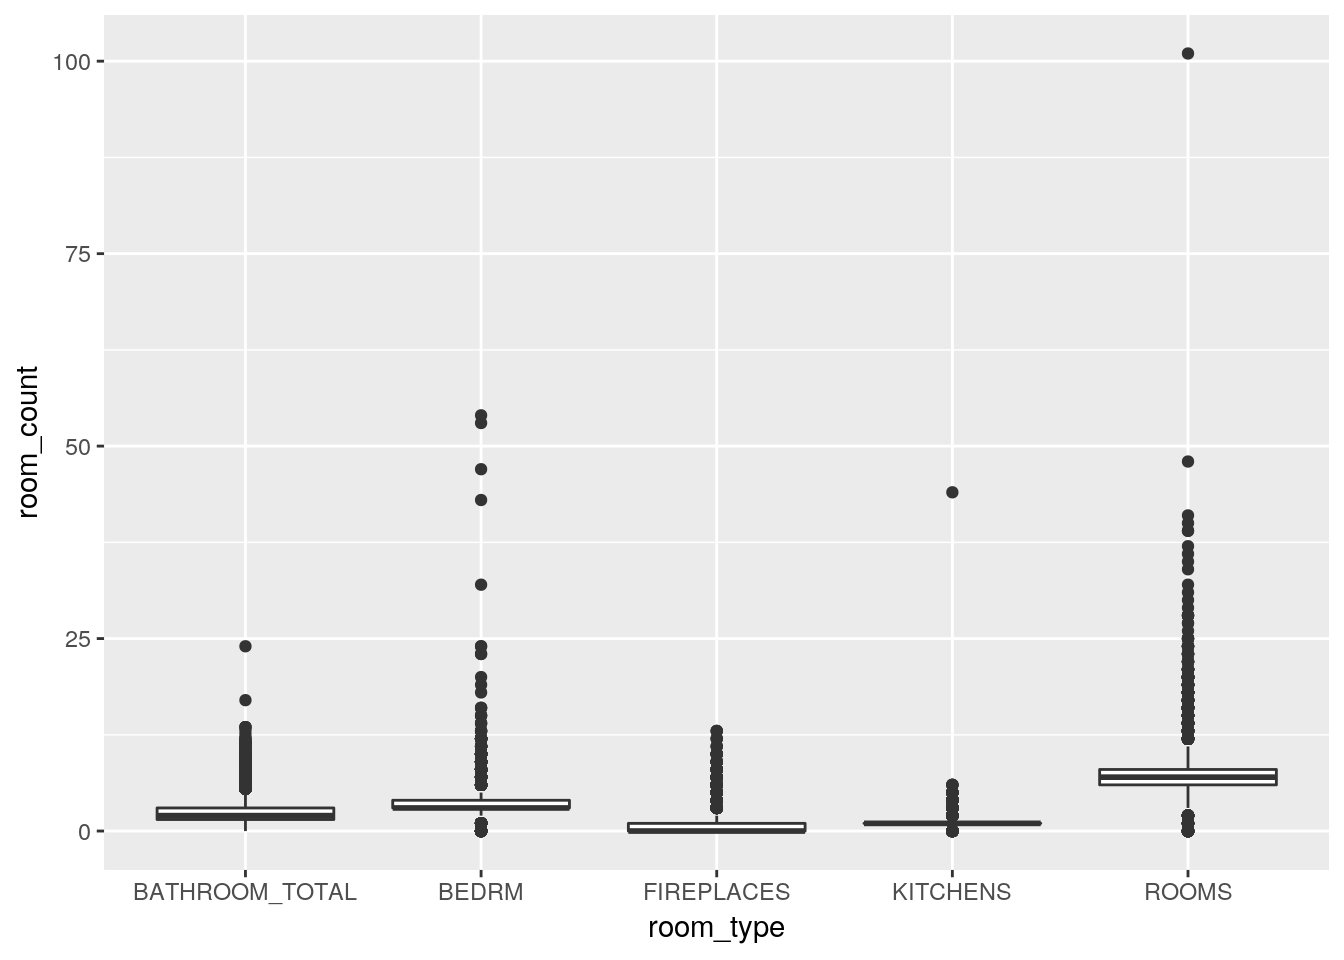
\includegraphics{Residential_Appraisal_files/figure-latex/EDA_rooms-1.pdf}
residence with 101 ROOMS is outlier. Let's investigate it.

\begin{Shaded}
\begin{Highlighting}[]
\NormalTok{residential_clean_df[residential_clean_df[}\StringTok{'ROOMS'}\NormalTok{] }\OperatorTok{==}\StringTok{ }\DecValTok{101}\NormalTok{,]}
\end{Highlighting}
\end{Shaded}

\begin{verbatim}
## # A tibble: 18 x 27
##    SSL       HEAT  AC    NUM_UNITS ROOMS BEDRM   AYB YR_RMDL   EYB STORIES
##    <chr>     <fct> <fct>     <int> <int> <int> <int>   <int> <int>   <dbl>
##  1 <NA>      <NA>  <NA>         NA    NA    NA    NA      NA    NA      NA
##  2 <NA>      <NA>  <NA>         NA    NA    NA    NA      NA    NA      NA
##  3 <NA>      <NA>  <NA>         NA    NA    NA    NA      NA    NA      NA
##  4 <NA>      <NA>  <NA>         NA    NA    NA    NA      NA    NA      NA
##  5 <NA>      <NA>  <NA>         NA    NA    NA    NA      NA    NA      NA
##  6 <NA>      <NA>  <NA>         NA    NA    NA    NA      NA    NA      NA
##  7 <NA>      <NA>  <NA>         NA    NA    NA    NA      NA    NA      NA
##  8 <NA>      <NA>  <NA>         NA    NA    NA    NA      NA    NA      NA
##  9 <NA>      <NA>  <NA>         NA    NA    NA    NA      NA    NA      NA
## 10 <NA>      <NA>  <NA>         NA    NA    NA    NA      NA    NA      NA
## 11 <NA>      <NA>  <NA>         NA    NA    NA    NA      NA    NA      NA
## 12 <NA>      <NA>  <NA>         NA    NA    NA    NA      NA    NA      NA
## 13 3304    ~ 13    0             1   101     3  1936    2006  1982       2
## 14 <NA>      <NA>  <NA>         NA    NA    NA    NA      NA    NA      NA
## 15 <NA>      <NA>  <NA>         NA    NA    NA    NA      NA    NA      NA
## 16 <NA>      <NA>  <NA>         NA    NA    NA    NA      NA    NA      NA
## 17 <NA>      <NA>  <NA>         NA    NA    NA    NA      NA    NA      NA
## 18 <NA>      <NA>  <NA>         NA    NA    NA    NA      NA    NA      NA
## # ... with 17 more variables: SALEDATE <dttm>, PRICE <int>,
## #   QUALIFIED <chr>, SALE_NUM <int>, GBA <int>, STYLE <fct>, STRUCT <fct>,
## #   GRADE <fct>, CNDTN <fct>, EXTWALL <fct>, ROOF <fct>, INTWALL <fct>,
## #   KITCHENS <int>, FIREPLACES <int>, LANDAREA <int>,
## #   BATHROOM_TOTAL <dbl>, LAND_USE <fct>
\end{verbatim}

\begin{Shaded}
\begin{Highlighting}[]
\CommentTok{# It seems to be fat fingure error. Rather ROOMS seems to be 10 looking at number of kitchens. bede room etc.}

\NormalTok{residential_clean_df[residential_clean_df}\OperatorTok{$}\NormalTok{SSL }\OperatorTok{==}\StringTok{ '3304    0041'}\NormalTok{,][}\StringTok{'ROOMS'}\NormalTok{] =}\StringTok{ }\DecValTok{10}

\CommentTok{# similarly KITCHENS with 44 seems to be typo instead of 4.}
\NormalTok{residential_clean_df[residential_clean_df}\OperatorTok{$}\NormalTok{SSL }\OperatorTok{==}\StringTok{ '4052    0129'}\NormalTok{,][}\StringTok{'KITCHENS'}\NormalTok{] =}\StringTok{ }\DecValTok{4}
\NormalTok{residential_clean_df[residential_clean_df}\OperatorTok{$}\NormalTok{BEDRM }\OperatorTok{>}\StringTok{ }\DecValTok{20}\NormalTok{,]}
\end{Highlighting}
\end{Shaded}

\begin{verbatim}
## # A tibble: 13 x 27
##    SSL       HEAT  AC    NUM_UNITS ROOMS BEDRM   AYB YR_RMDL   EYB STORIES
##    <chr>     <fct> <fct>     <int> <dbl> <int> <int>   <int> <int>   <dbl>
##  1 <NA>      <NA>  <NA>         NA    NA    NA    NA      NA    NA    NA  
##  2 <NA>      <NA>  <NA>         NA    NA    NA    NA      NA    NA    NA  
##  3 1399    ~ 1     1             1    11    53  1940    1999  1972     2  
##  4 1388    ~ 7     1             1     6    32  1940    1998  1969     2  
##  5 2232    ~ 1     1             1    48    24  1990    2009  2010     2  
##  6 2700    ~ 13    0             1     7    43  1915    2014  1969     2  
##  7 2638    ~ 1     1             1     7    47  1947      NA  1963     2.5
##  8 2865    ~ 13    1             1     6    54  1910    2004  1967     2  
##  9 3339    ~ 13    0             1     5    23  1925      NA  1954     1  
## 10 <NA>      <NA>  <NA>         NA    NA    NA    NA      NA    NA    NA  
## 11 3653    ~ 1     1             4    36    24  2014      NA  2015     3  
## 12 <NA>      <NA>  <NA>         NA    NA    NA    NA      NA    NA    NA  
## 13 5130    ~ 13    0             1     5    23  1945      NA  1945     2  
## # ... with 17 more variables: SALEDATE <dttm>, PRICE <int>,
## #   QUALIFIED <chr>, SALE_NUM <int>, GBA <int>, STYLE <fct>, STRUCT <fct>,
## #   GRADE <fct>, CNDTN <fct>, EXTWALL <fct>, ROOF <fct>, INTWALL <fct>,
## #   KITCHENS <dbl>, FIREPLACES <int>, LANDAREA <int>,
## #   BATHROOM_TOTAL <dbl>, LAND_USE <fct>
\end{verbatim}

\hypertarget{year-variables.}{%
\subsection{Year variables.}\label{year-variables.}}

AYB - Actual year built.\\
EYB - Estimated year built.\\
YR\_RMDL - Year remodelled.\\
SaleDate - Sale of the residential property. Rationale of feature
engineering.\\
1. Take into account the depreciation. Calculate AGe of residential
property at the time of sale.\\
2. Age can be calculated by sale\_year - max(AYB, EYB, YR\_RMDL)\\
3. there should be differentiation of property remodelled vs newly buit
in the same year. Create one variable (factor) if the property is
remodelled.

\begin{Shaded}
\begin{Highlighting}[]
\CommentTok{# extract sale year. 1900 is coded for not sold residences. mutating these records to 2018 to predict the sale for current year}
\NormalTok{residential_clean_df <-}\StringTok{ }\NormalTok{residential_clean_df }\OperatorTok
\StringTok{  }\KeywordTok{mutate}\NormalTok{(}\DataTypeTok{sale_year =}  \KeywordTok{if_else}\NormalTok{(}\KeywordTok{year}\NormalTok{(residential_clean_df}\OperatorTok{$}\NormalTok{SALEDATE)}\OperatorTok{==}\DecValTok{1900}\NormalTok{,}\DecValTok{2018}\NormalTok{,}
                              \KeywordTok{year}\NormalTok{(residential_clean_df}\OperatorTok{$}\NormalTok{SALEDATE)))}

\CommentTok{# to check if the remodelling is done and ppulate the variable. Some of the remodelling happened after the sale date.We need to check if the remodelling happened before sale date to populare remodelled flag.}
\NormalTok{residential_clean_df <-}\StringTok{ }\NormalTok{residential_clean_df }\OperatorTok
\StringTok{  }\KeywordTok{mutate}\NormalTok{(}\DataTypeTok{yr_remod_mod =} \KeywordTok{if_else}\NormalTok{(}\KeywordTok{is.na}\NormalTok{(YR_RMDL),}\DecValTok{2018}\NormalTok{,}\KeywordTok{as.numeric}\NormalTok{(YR_RMDL))) }\OperatorTok
\StringTok{  }\KeywordTok{mutate}\NormalTok{(}\DataTypeTok{remodelled =} \KeywordTok{as.factor}\NormalTok{(}\KeywordTok{if_else}\NormalTok{(yr_remod_mod }\OperatorTok{<}\StringTok{ }\NormalTok{sale_year,}\DecValTok{1}\NormalTok{,}\DecValTok{0}\NormalTok{))) }\OperatorTok
\StringTok{  }\KeywordTok{select}\NormalTok{(}\OperatorTok{-}\NormalTok{yr_remod_mod)}

\CommentTok{# calculate age variable which is as of sale year.}
\NormalTok{residential_clean_df <-}\StringTok{ }\NormalTok{residential_clean_df }\OperatorTok
\StringTok{  }\KeywordTok{mutate}\NormalTok{(}\DataTypeTok{age =} \KeywordTok{pmin}\NormalTok{(}\KeywordTok{if_else}\NormalTok{(sale_year }\OperatorTok{-}\StringTok{ }\NormalTok{AYB }\OperatorTok{<}\DecValTok{0}\NormalTok{, }\DecValTok{999}\NormalTok{,  sale_year }\OperatorTok{-}\StringTok{ }\NormalTok{AYB ),}
                    \KeywordTok{if_else}\NormalTok{(sale_year }\OperatorTok{-}\StringTok{ }\NormalTok{EYB }\OperatorTok{<}\DecValTok{0}\NormalTok{, }\DecValTok{999}\NormalTok{,  sale_year }\OperatorTok{-}\StringTok{ }\NormalTok{EYB ), }
                    \KeywordTok{if_else}\NormalTok{(sale_year }\OperatorTok{-}\StringTok{ }\NormalTok{YR_RMDL }\OperatorTok{<}\DecValTok{0}\NormalTok{, }\DecValTok{999}\NormalTok{,  sale_year }\OperatorTok{-}\StringTok{ }\NormalTok{YR_RMDL ), }
                    \DataTypeTok{na.rm=}\OtherTok{TRUE}\NormalTok{))}

\CommentTok{# excluding the date columns}
\NormalTok{residential_clean_df <-}\StringTok{ }\NormalTok{residential_clean_df }\OperatorTok
\StringTok{  }\KeywordTok{select}\NormalTok{(}\OperatorTok{-}\NormalTok{AYB, }\OperatorTok{-}\NormalTok{EYB, }\OperatorTok{-}\NormalTok{YR_RMDL, }\OperatorTok{-}\NormalTok{SALEDATE)}
\end{Highlighting}
\end{Shaded}

\hypertarget{analyse-area}{%
\subsubsection{Analyse area}\label{analyse-area}}

GBA and LandAREA.

\begin{Shaded}
\begin{Highlighting}[]
\NormalTok{residential_clean_df }\OperatorTok
\StringTok{  }\KeywordTok{select}\NormalTok{(GBA,LANDAREA) }\OperatorTok
\StringTok{  }\KeywordTok{gather}\NormalTok{(}\DataTypeTok{key =} \StringTok{'type'}\NormalTok{, }\DataTypeTok{value =} \StringTok{'area'}\NormalTok{) }\OperatorTok
\StringTok{  }\KeywordTok{ggplot}\NormalTok{(}\DataTypeTok{data =}\NormalTok{ ., }\KeywordTok{aes}\NormalTok{(}\DataTypeTok{x =}\NormalTok{ type, }\DataTypeTok{y =}\NormalTok{ area)) }\OperatorTok{+}
\StringTok{  }\KeywordTok{geom_boxplot}\NormalTok{()}
\end{Highlighting}
\end{Shaded}

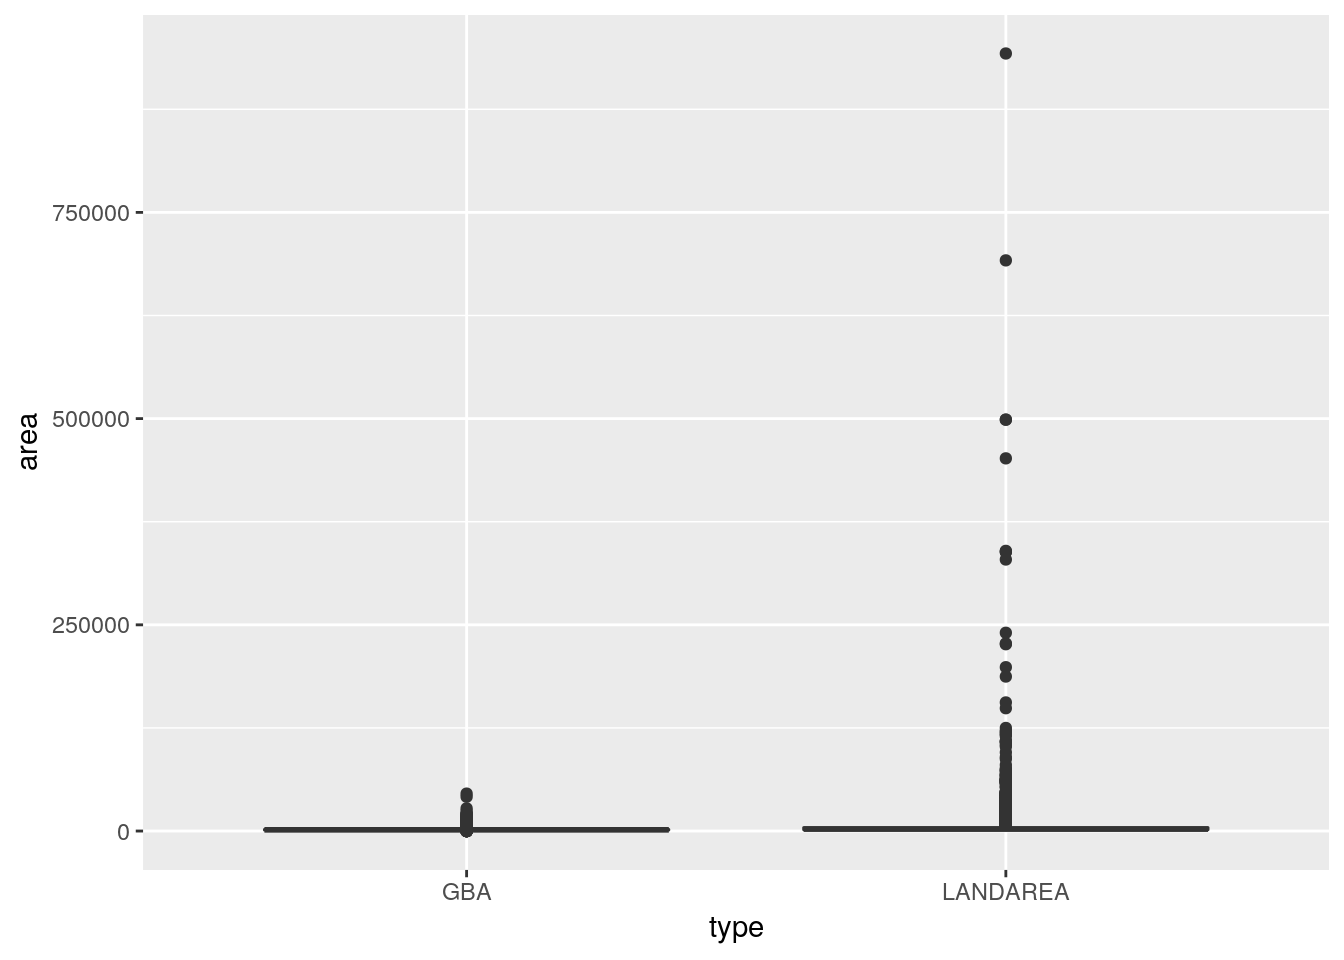
\includegraphics{Residential_Appraisal_files/figure-latex/EDA_AREA-1.pdf}

\begin{Shaded}
\begin{Highlighting}[]
\CommentTok{#below are some extreme values from area perspective. However they seems valid numbers}
\NormalTok{residential_clean_df[residential_clean_df}\OperatorTok{$}\NormalTok{GBA }\OperatorTok{>}\StringTok{ }\DecValTok{40000}\NormalTok{,]}
\end{Highlighting}
\end{Shaded}

\begin{verbatim}
## # A tibble: 2 x 26
##   SSL   HEAT  AC    NUM_UNITS ROOMS BEDRM STORIES PRICE QUALIFIED SALE_NUM
##   <chr> <fct> <fct>     <int> <dbl> <int>   <dbl> <int> <chr>        <int>
## 1 1640~ 7     1             1    18     5     2.5    NA U                1
## 2 2147~ 7     1             1    40    10     2      NA U                1
## # ... with 16 more variables: GBA <int>, STYLE <fct>, STRUCT <fct>,
## #   GRADE <fct>, CNDTN <fct>, EXTWALL <fct>, ROOF <fct>, INTWALL <fct>,
## #   KITCHENS <dbl>, FIREPLACES <int>, LANDAREA <int>,
## #   BATHROOM_TOTAL <dbl>, LAND_USE <fct>, sale_year <dbl>,
## #   remodelled <fct>, age <dbl>
\end{verbatim}

\begin{Shaded}
\begin{Highlighting}[]
\NormalTok{residential_clean_df[residential_clean_df}\OperatorTok{$}\NormalTok{LANDAREA }\OperatorTok{>}\StringTok{ }\DecValTok{500000}\NormalTok{,]}
\end{Highlighting}
\end{Shaded}

\begin{verbatim}
## # A tibble: 2 x 26
##   SSL   HEAT  AC    NUM_UNITS ROOMS BEDRM STORIES PRICE QUALIFIED SALE_NUM
##   <chr> <fct> <fct>     <int> <dbl> <int>   <dbl> <int> <chr>        <int>
## 1 2248~ 13    1             1    34     7    2.75     0 U                1
## 2 2630~ 7     1             1    39    12    3        0 U                4
## # ... with 16 more variables: GBA <int>, STYLE <fct>, STRUCT <fct>,
## #   GRADE <fct>, CNDTN <fct>, EXTWALL <fct>, ROOF <fct>, INTWALL <fct>,
## #   KITCHENS <dbl>, FIREPLACES <int>, LANDAREA <int>,
## #   BATHROOM_TOTAL <dbl>, LAND_USE <fct>, sale_year <dbl>,
## #   remodelled <fct>, age <dbl>
\end{verbatim}

Lets bucket land area and GBA into 5 groups each based on quartiles.

\begin{Shaded}
\begin{Highlighting}[]
\NormalTok{residential_clean_df <-}\StringTok{ }\NormalTok{residential_clean_df }\OperatorTok
\StringTok{  }\KeywordTok{mutate}\NormalTok{(}\DataTypeTok{GBA_Bucket =} \KeywordTok{case_when}\NormalTok{(GBA }\OperatorTok{<=}\StringTok{ }\KeywordTok{quantile}\NormalTok{(GBA,}\DataTypeTok{probs=}\KeywordTok{c}\NormalTok{(}\FloatTok{0.25}\NormalTok{)) }\OperatorTok{~}\StringTok{ }\DecValTok{0}\NormalTok{,}
\NormalTok{                                GBA }\OperatorTok{<=}\StringTok{ }\KeywordTok{median}\NormalTok{(GBA, }\DataTypeTok{na.rm =} \OtherTok{TRUE}\NormalTok{) }\OperatorTok{~}\DecValTok{1}\NormalTok{,}
\NormalTok{                                GBA }\OperatorTok{<=}\StringTok{ }\KeywordTok{quantile}\NormalTok{(GBA,}\DataTypeTok{probs=}\KeywordTok{c}\NormalTok{(}\FloatTok{0.75}\NormalTok{)) }\OperatorTok{~}\StringTok{ }\DecValTok{2}\NormalTok{,}
\NormalTok{                                GBA }\OperatorTok{<=}\StringTok{ }\KeywordTok{quantile}\NormalTok{(GBA,}\DataTypeTok{probs=}\KeywordTok{c}\NormalTok{(}\FloatTok{0.90}\NormalTok{)) }\OperatorTok{~}\StringTok{ }\DecValTok{3}\NormalTok{,}
\NormalTok{                                GBA }\OperatorTok{>}\StringTok{ }\KeywordTok{quantile}\NormalTok{(GBA,}\DataTypeTok{probs=}\KeywordTok{c}\NormalTok{(}\FloatTok{0.90}\NormalTok{)) }\OperatorTok{~}\StringTok{ }\DecValTok{4}\NormalTok{)) }\OperatorTok
\StringTok{  }\KeywordTok{mutate}\NormalTok{(}\DataTypeTok{LANDAREA_Bucket =} \KeywordTok{case_when}\NormalTok{(LANDAREA }\OperatorTok{<=}\StringTok{ }\KeywordTok{quantile}\NormalTok{(LANDAREA,}\DataTypeTok{probs=}\KeywordTok{c}\NormalTok{(}\FloatTok{0.25}\NormalTok{)) }\OperatorTok{~}\StringTok{ }\DecValTok{0}\NormalTok{,}
\NormalTok{                                LANDAREA }\OperatorTok{<=}\StringTok{ }\KeywordTok{median}\NormalTok{(LANDAREA, }\DataTypeTok{na.rm =} \OtherTok{TRUE}\NormalTok{) }\OperatorTok{~}\DecValTok{1}\NormalTok{,}
\NormalTok{                                LANDAREA }\OperatorTok{<=}\StringTok{ }\KeywordTok{quantile}\NormalTok{(LANDAREA,}\DataTypeTok{probs=}\KeywordTok{c}\NormalTok{(}\FloatTok{0.75}\NormalTok{)) }\OperatorTok{~}\StringTok{ }\DecValTok{2}\NormalTok{,}
\NormalTok{                                LANDAREA }\OperatorTok{<=}\StringTok{ }\KeywordTok{quantile}\NormalTok{(LANDAREA,}\DataTypeTok{probs=}\KeywordTok{c}\NormalTok{(}\FloatTok{0.90}\NormalTok{)) }\OperatorTok{~}\StringTok{ }\DecValTok{3}\NormalTok{,}
\NormalTok{                                LANDAREA }\OperatorTok{>}\StringTok{ }\KeywordTok{quantile}\NormalTok{(LANDAREA,}\DataTypeTok{probs=}\KeywordTok{c}\NormalTok{(}\FloatTok{0.90}\NormalTok{)) }\OperatorTok{~}\StringTok{ }\DecValTok{4}\NormalTok{))}
\CommentTok{# remove LAND_AREA and GBA}
\NormalTok{residential_clean_df <-}\StringTok{ }\NormalTok{residential_clean_df }\OperatorTok
\StringTok{  }\KeywordTok{select}\NormalTok{(}\OperatorTok{-}\KeywordTok{c}\NormalTok{(LANDAREA, GBA, SALE_NUM))}
\end{Highlighting}
\end{Shaded}

\hypertarget{test-and-train-dataset.}{%
\subsection{Test and train dataset.}\label{test-and-train-dataset.}}

SALES QUALIFICATION The basic sales information is available at the
Register of Deeds. However, before a proper analysis can be made between
the sales for the tax year and those of similar properties that did not
sell, the sales must be checked or qualified to verify that and ``arm's
length'' transaction has taken place and the source of information is
correct. The transaction must then be further checked to determine if
all rights and benefits of property ownership were transferred and if
any personal property was involved. This procedure is known as SALES
QUALIFICATION. Sales of some residential, but primarily agricultural,
industrial and commercial properties often include personal property.
There are also a number of intra-company or intra-family transfers
``distress'' sales, etc., many of which have limiting terms and
conditions which affect the sales price. For these reasons and others,
further qualification of sales of this type through communication with
one or more of the parties involved may be necessary to determine if the
sales price should be adjusted for terms, personal property, etc., or
disqualified entirely.

\begin{Shaded}
\begin{Highlighting}[]
\NormalTok{residential_clean_df }\OperatorTok\StringTok{ }
\StringTok{  }\KeywordTok{filter}\NormalTok{(QUALIFIED }\OperatorTok{==}\StringTok{ 'Q'}\NormalTok{) }\OperatorTok
\StringTok{  }\KeywordTok{select}\NormalTok{(PRICE) }\OperatorTok
\StringTok{  }\KeywordTok{summary}\NormalTok{()}
\end{Highlighting}
\end{Shaded}

\begin{verbatim}
##      PRICE         
##  Min.   :       0  
##  1st Qu.:  289900  
##  Median :  507000  
##  Mean   :  628358  
##  3rd Qu.:  800000  
##  Max.   :22000000  
##  NA's   :1
\end{verbatim}

\begin{Shaded}
\begin{Highlighting}[]
\CommentTok{# cross check NA price and 0 price for qualified sales.}
\NormalTok{residential_clean_df }\OperatorTok
\StringTok{  }\KeywordTok{filter}\NormalTok{(QUALIFIED }\OperatorTok{==}\StringTok{ 'Q'}\NormalTok{, }\KeywordTok{is.na}\NormalTok{(PRICE))}
\end{Highlighting}
\end{Shaded}

\begin{verbatim}
## # A tibble: 1 x 25
##   SSL      HEAT  AC    NUM_UNITS ROOMS BEDRM STORIES PRICE QUALIFIED STYLE
##   <chr>    <fct> <fct>     <int> <dbl> <int>   <dbl> <int> <chr>     <fct>
## 1 3986   ~ 7     1             1     7     3       2    NA Q         4    
## # ... with 15 more variables: STRUCT <fct>, GRADE <fct>, CNDTN <fct>,
## #   EXTWALL <fct>, ROOF <fct>, INTWALL <fct>, KITCHENS <dbl>,
## #   FIREPLACES <int>, BATHROOM_TOTAL <dbl>, LAND_USE <fct>,
## #   sale_year <dbl>, remodelled <fct>, age <dbl>, GBA_Bucket <dbl>,
## #   LANDAREA_Bucket <dbl>
\end{verbatim}

\begin{Shaded}
\begin{Highlighting}[]
\NormalTok{residential_clean_df }\OperatorTok
\StringTok{  }\KeywordTok{filter}\NormalTok{(QUALIFIED }\OperatorTok{==}\StringTok{ 'Q'}\NormalTok{,PRICE }\OperatorTok{==}\StringTok{ }\DecValTok{0}\NormalTok{)}
\end{Highlighting}
\end{Shaded}

\begin{verbatim}
## # A tibble: 88 x 25
##    SSL     HEAT  AC    NUM_UNITS ROOMS BEDRM STORIES PRICE QUALIFIED STYLE
##    <chr>   <fct> <fct>     <int> <dbl> <int>   <dbl> <int> <chr>     <fct>
##  1 0193  ~ 7     1             4    16     8       3     0 Q         7    
##  2 0110  ~ 13    0             1     8     4       2     0 Q         4    
##  3 0237  ~ 13    0             2    10     3       2     0 Q         4    
##  4 0241  ~ 8     1             4    14     6       3     0 Q         7    
##  5 0206  ~ 7     1             1     6     3       2     0 Q         4    
##  6 0357  ~ 1     0             1     5     2       2     0 Q         4    
##  7 0617  ~ 13    0             1     6     3       2     0 Q         4    
##  8 0513  ~ 1     1             1     8     4       3     0 Q         7    
##  9 0834  ~ 7     1             2     9     4       2     0 Q         4    
## 10 0877  ~ 1     1             2     8     2       2     0 Q         4    
## # ... with 78 more rows, and 15 more variables: STRUCT <fct>, GRADE <fct>,
## #   CNDTN <fct>, EXTWALL <fct>, ROOF <fct>, INTWALL <fct>, KITCHENS <dbl>,
## #   FIREPLACES <int>, BATHROOM_TOTAL <dbl>, LAND_USE <fct>,
## #   sale_year <dbl>, remodelled <fct>, age <dbl>, GBA_Bucket <dbl>,
## #   LANDAREA_Bucket <dbl>
\end{verbatim}

\begin{Shaded}
\begin{Highlighting}[]
\CommentTok{# these records need to be removed and missing values.}

\NormalTok{residential_clean_df <-}\StringTok{ }\NormalTok{residential_clean_df }\OperatorTok
\StringTok{  }\KeywordTok{filter}\NormalTok{(QUALIFIED }\OperatorTok{==}\StringTok{ 'Q'}\NormalTok{, }\OperatorTok{!}\KeywordTok{is.na}\NormalTok{(PRICE))}

\NormalTok{residential_clean_df <-}\StringTok{ }\NormalTok{residential_clean_df }\OperatorTok
\StringTok{  }\KeywordTok{filter}\NormalTok{(QUALIFIED }\OperatorTok{==}\StringTok{ 'Q'}\NormalTok{, PRICE }\OperatorTok{!=}\StringTok{ }\DecValTok{0}\NormalTok{)}

\NormalTok{residential_clean_df }\OperatorTok
\StringTok{  }\KeywordTok{filter}\NormalTok{(QUALIFIED }\OperatorTok{==}\StringTok{ 'Q'}\NormalTok{) }\OperatorTok
\StringTok{  }\KeywordTok{select}\NormalTok{(PRICE) }\OperatorTok
\StringTok{  }\KeywordTok{ggplot}\NormalTok{(}\DataTypeTok{data =}\NormalTok{ ., }\KeywordTok{aes}\NormalTok{(}\DataTypeTok{x=}\NormalTok{PRICE)) }\OperatorTok{+}
\StringTok{  }\KeywordTok{geom_histogram}\NormalTok{(}\DataTypeTok{bins =} \DecValTok{60}\NormalTok{)}
\end{Highlighting}
\end{Shaded}

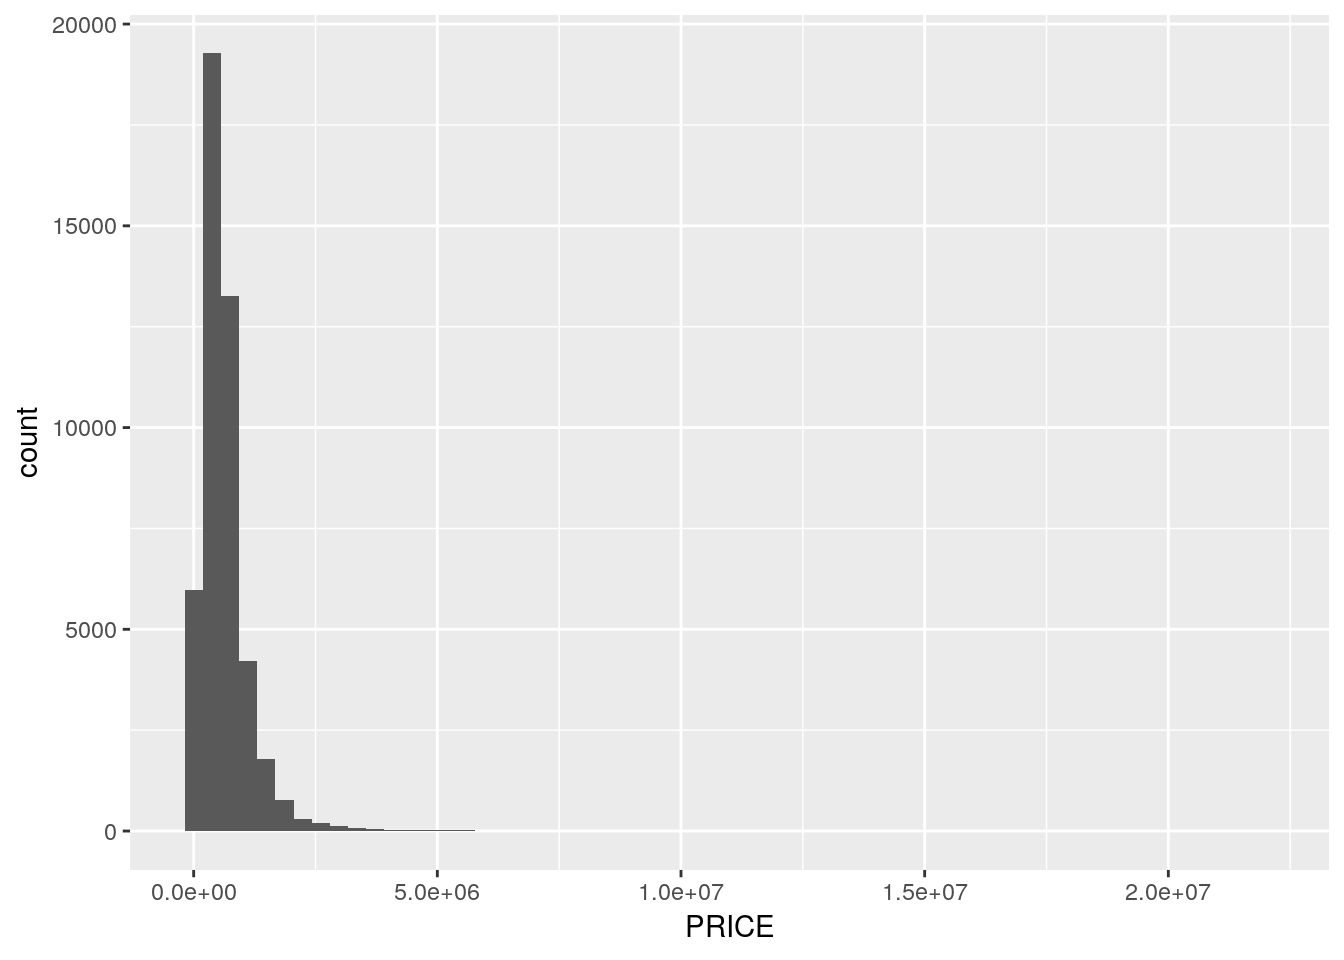
\includegraphics{Residential_Appraisal_files/figure-latex/data_prep-1.pdf}

\begin{Shaded}
\begin{Highlighting}[]
\KeywordTok{summary}\NormalTok{(residential_clean_df)}
\end{Highlighting}
\end{Shaded}

\begin{verbatim}
##      SSL                 HEAT       AC          NUM_UNITS    
##  Length:46201       1      :18278   0:10693   Min.   :0.000  
##  Class :character   13     :15220   1:35508   1st Qu.:1.000  
##  Mode  :character   7      :11722             Median :1.000  
##                     8      :  667             Mean   :1.195  
##                     6      :   80             3rd Qu.:1.000  
##                     3      :   57             Max.   :6.000  
##                     (Other):  177                            
##      ROOMS           BEDRM           STORIES            PRICE         
##  Min.   : 0.00   Min.   : 0.000   Min.   :  0.000   Min.   :     250  
##  1st Qu.: 6.00   1st Qu.: 3.000   1st Qu.:  2.000   1st Qu.:  290000  
##  Median : 7.00   Median : 3.000   Median :  2.000   Median :  510000  
##  Mean   : 7.41   Mean   : 3.435   Mean   :  2.137   Mean   :  629555  
##  3rd Qu.: 8.00   3rd Qu.: 4.000   3rd Qu.:  2.000   3rd Qu.:  800000  
##  Max.   :28.00   Max.   :53.000   Max.   :826.000   Max.   :22000000  
##  NA's   :9       NA's   :2        NA's   :28                          
##   QUALIFIED             STYLE           STRUCT          GRADE      
##  Length:46201       4      :35135   7      :19164   3      :14589  
##  Class :character   7      : 4615   1      :12950   4      :13759  
##  Mode  :character   6      : 3329   8      : 6539   5      : 9907  
##                     1      : 1408   6      : 5572   6      : 4388  
##                     3      :  855   2      : 1755   7      : 1591  
##                     5      :  306   5      :  154   8      : 1325  
##                     (Other):  553   (Other):   67   (Other):  642  
##  CNDTN        EXTWALL           ROOF          INTWALL         KITCHENS    
##  0:    1   14     :34714   2      :13731   6      :35626   Min.   :0.000  
##  1:   32   22     : 2937   6      :13112   11     : 6064   1st Qu.:1.000  
##  2:  231   4      : 2349   1      :12831   3      : 2952   Median :1.000  
##  3:16915   6      : 1781   11     : 4709   2      : 1422   Mean   :1.229  
##  4:22081   5      : 1306   13     :  798   10     :   37   3rd Qu.:1.000  
##  5: 6160   10     :  484   4      :  308   4      :   36   Max.   :6.000  
##  6:  781   (Other): 2630   (Other):  712   (Other):   64   NA's   :1      
##    FIREPLACES      BATHROOM_TOTAL  LAND_USE    sale_year    remodelled
##  Min.   : 0.0000   Min.   : 0.00   0:40414   Min.   :1982   0:29527   
##  1st Qu.: 0.0000   1st Qu.: 2.00   1: 5787   1st Qu.:2004   1:16674   
##  Median : 0.0000   Median : 2.50             Median :2011             
##  Mean   : 0.6815   Mean   : 2.59             Mean   :2009             
##  3rd Qu.: 1.0000   3rd Qu.: 3.50             3rd Qu.:2015             
##  Max.   :13.0000   Max.   :13.50             Max.   :2018             
##  NA's   :1                                                            
##       age           GBA_Bucket    LANDAREA_Bucket
##  Min.   :  0.00   Min.   :0.000   Min.   :0.00   
##  1st Qu.:  1.00   1st Qu.:1.000   1st Qu.:0.00   
##  Median : 12.00   Median :2.000   Median :1.00   
##  Mean   : 24.14   Mean   :1.653   Mean   :1.49   
##  3rd Qu.: 41.00   3rd Qu.:3.000   3rd Qu.:2.00   
##  Max.   :999.00   Max.   :4.000   Max.   :4.00   
## 
\end{verbatim}


\end{document}
